\documentclass[conference]{IEEEtran}

\input epsf
\usepackage{graphicx}
\usepackage{gensymb}
\usepackage{subfigure}
\usepackage{algorithm}
\usepackage{algpseudocode}
\usepackage{booktabs}
\usepackage{url}

\ifCLASSOPTIONcompsoc
    \usepackage[nocompress]{cite}
\else
    \usepackage{cite}
\fi

\renewcommand{\algorithmicrequire}{\textbf{Input:}}
\renewcommand{\algorithmicensure}{\textbf{Result:}}

\hyphenation{op-tical net-works semi-conduc-tor IEEEtran}

\begin{document}

\title{Precise Epidemic Control Based on GeoHash}

\author{
    Youwei Huang$^{1}$, Feng Lu$^{2,*}$, Xiaolong Sang$^{1}$, Bin Hu$^{2}$, Jiachun Tao$^{1}$
    \\
    \normalsize $^{1}$Institute of Intelligent Computing Technology, Suzhou, CAS
    \\
    \normalsize $^{2}$Institute of Computing Technology, Chinese Academy of Sciences
    \\
    \normalsize huangyw@iict.ac.cn, lufeng20g@ict.ac.cn
    \\
    \normalsize *Corresponding Author
}

\maketitle

\begin{abstract}
    Coronavirus Disease 2019 (COVID-19) is a highly transmissible and pathogenic coronavirus that emerged in late 2019 and has caused a pandemic of acute respiratory disease.
    Before vaccines are widely used or the invention of specific medication, many measures have been taken by human beings to prevent the spread of the epidemic.
    Quarantining infected groups and locking down high-risk regions are common means used by the latest medical experience.
    As such measures are generally carried out under administrative divisions, issues of imprecise epidemic control and unquantifiable risk warning are exposed gradually.
    In order to better achieve the purpose of precise epidemic prevention and control, we propose a kind of dynamic block division technology based on GeoHash which can be used to monitor, mark out and control the epidemic regions.
    By using GeoHash, we divide the earth map into connected dynamic blocks.
    Dynamic blocks are easily visualized in geographic information systems (GIS) equipped in electronic devices.
    GeoHash blocks are dynamically overlaid on the map as grids.
    Each block contains essential epidemic-related data and important features which are concerned by professional medical work.
    Quantitative analysis of epidemic data is carried out on each block.
    Our research shows the analysis results can support decision-making, measures formulation, and effectiveness assessment of COVID-19 prevention and control.
    Such research can be applied not only to COVID-19 but also to other infectious diseases.
\end{abstract}
\IEEEoverridecommandlockouts
\begin{keywords}
    GeoHash, 2019 novel coronavirus, COVID-19, GIS, ASI, precise epidemic control and prevent.
\end{keywords}

\IEEEpeerreviewmaketitle

\section{Introduction}
During the COVID-19\cite{hu2020characteristics} pandemic, many cities over the world were forced to lock down.
Wuhan city and the major cities in Hubei, China were put under lockdown on the 23rd and 24th Jan. 2020 respectively\cite{lau2020positive}.
Lockdown means a whole region is quarantined and cut off physical contact with outside.
Citizens are forbidden to leave their city or even their home.
The national medical team carries out centralized medical observation and treatment in quarantined regions.
Research shows, COVID-19 spread becomes weaker following lockdown\cite{lau2020positive}.
However the lockdown of a city can cause huge economic losses.
The lockdown of some vital areas can cause irreparable losses, such as financial center, political center, and industrial dependent cities.
Another issue that confuses people is how to distinguish whether the area they are in or where they are going is safe.
The current regional risk warning or lockdown is based on the administrative divisions as Fig. 1.
Cities, states or provinces, nations all over the world have different sizes and irregular geographic borders.
There may be an outbreak in a city, but it does not mean that the virus has spread to all corners of the city.
On the contrary, there may be no epidemic in the center of neighboring cities, but there is already a huge risk at the border of these cities.
As an example, Fig. 1 is a map that shows the initial locked down cities in Hubei province, China, a white block surrounded by red blocks was dangerous, even if it was not locked down at that time.
We summarize some weaknesses of current lockdown measures:
\begin{enumerate}
    \item The border of a city is irregular while the transmission of virus doesn't follow the administrative division.
    \item The administrative range of a region is constant, but the disease is spreadable, thus the lockdown areas are not expandable flexibly.
    \item Due to policy differences in different regions, information release is not complete and coincident.
    \item The news released by the local government may lag behind, thus it is difficult for residents to obtain the news in real time.
    \item A complete lockdown can lead to huge social and economic losses.
\end{enumerate}

\begin{figure}[h]
    \centering
    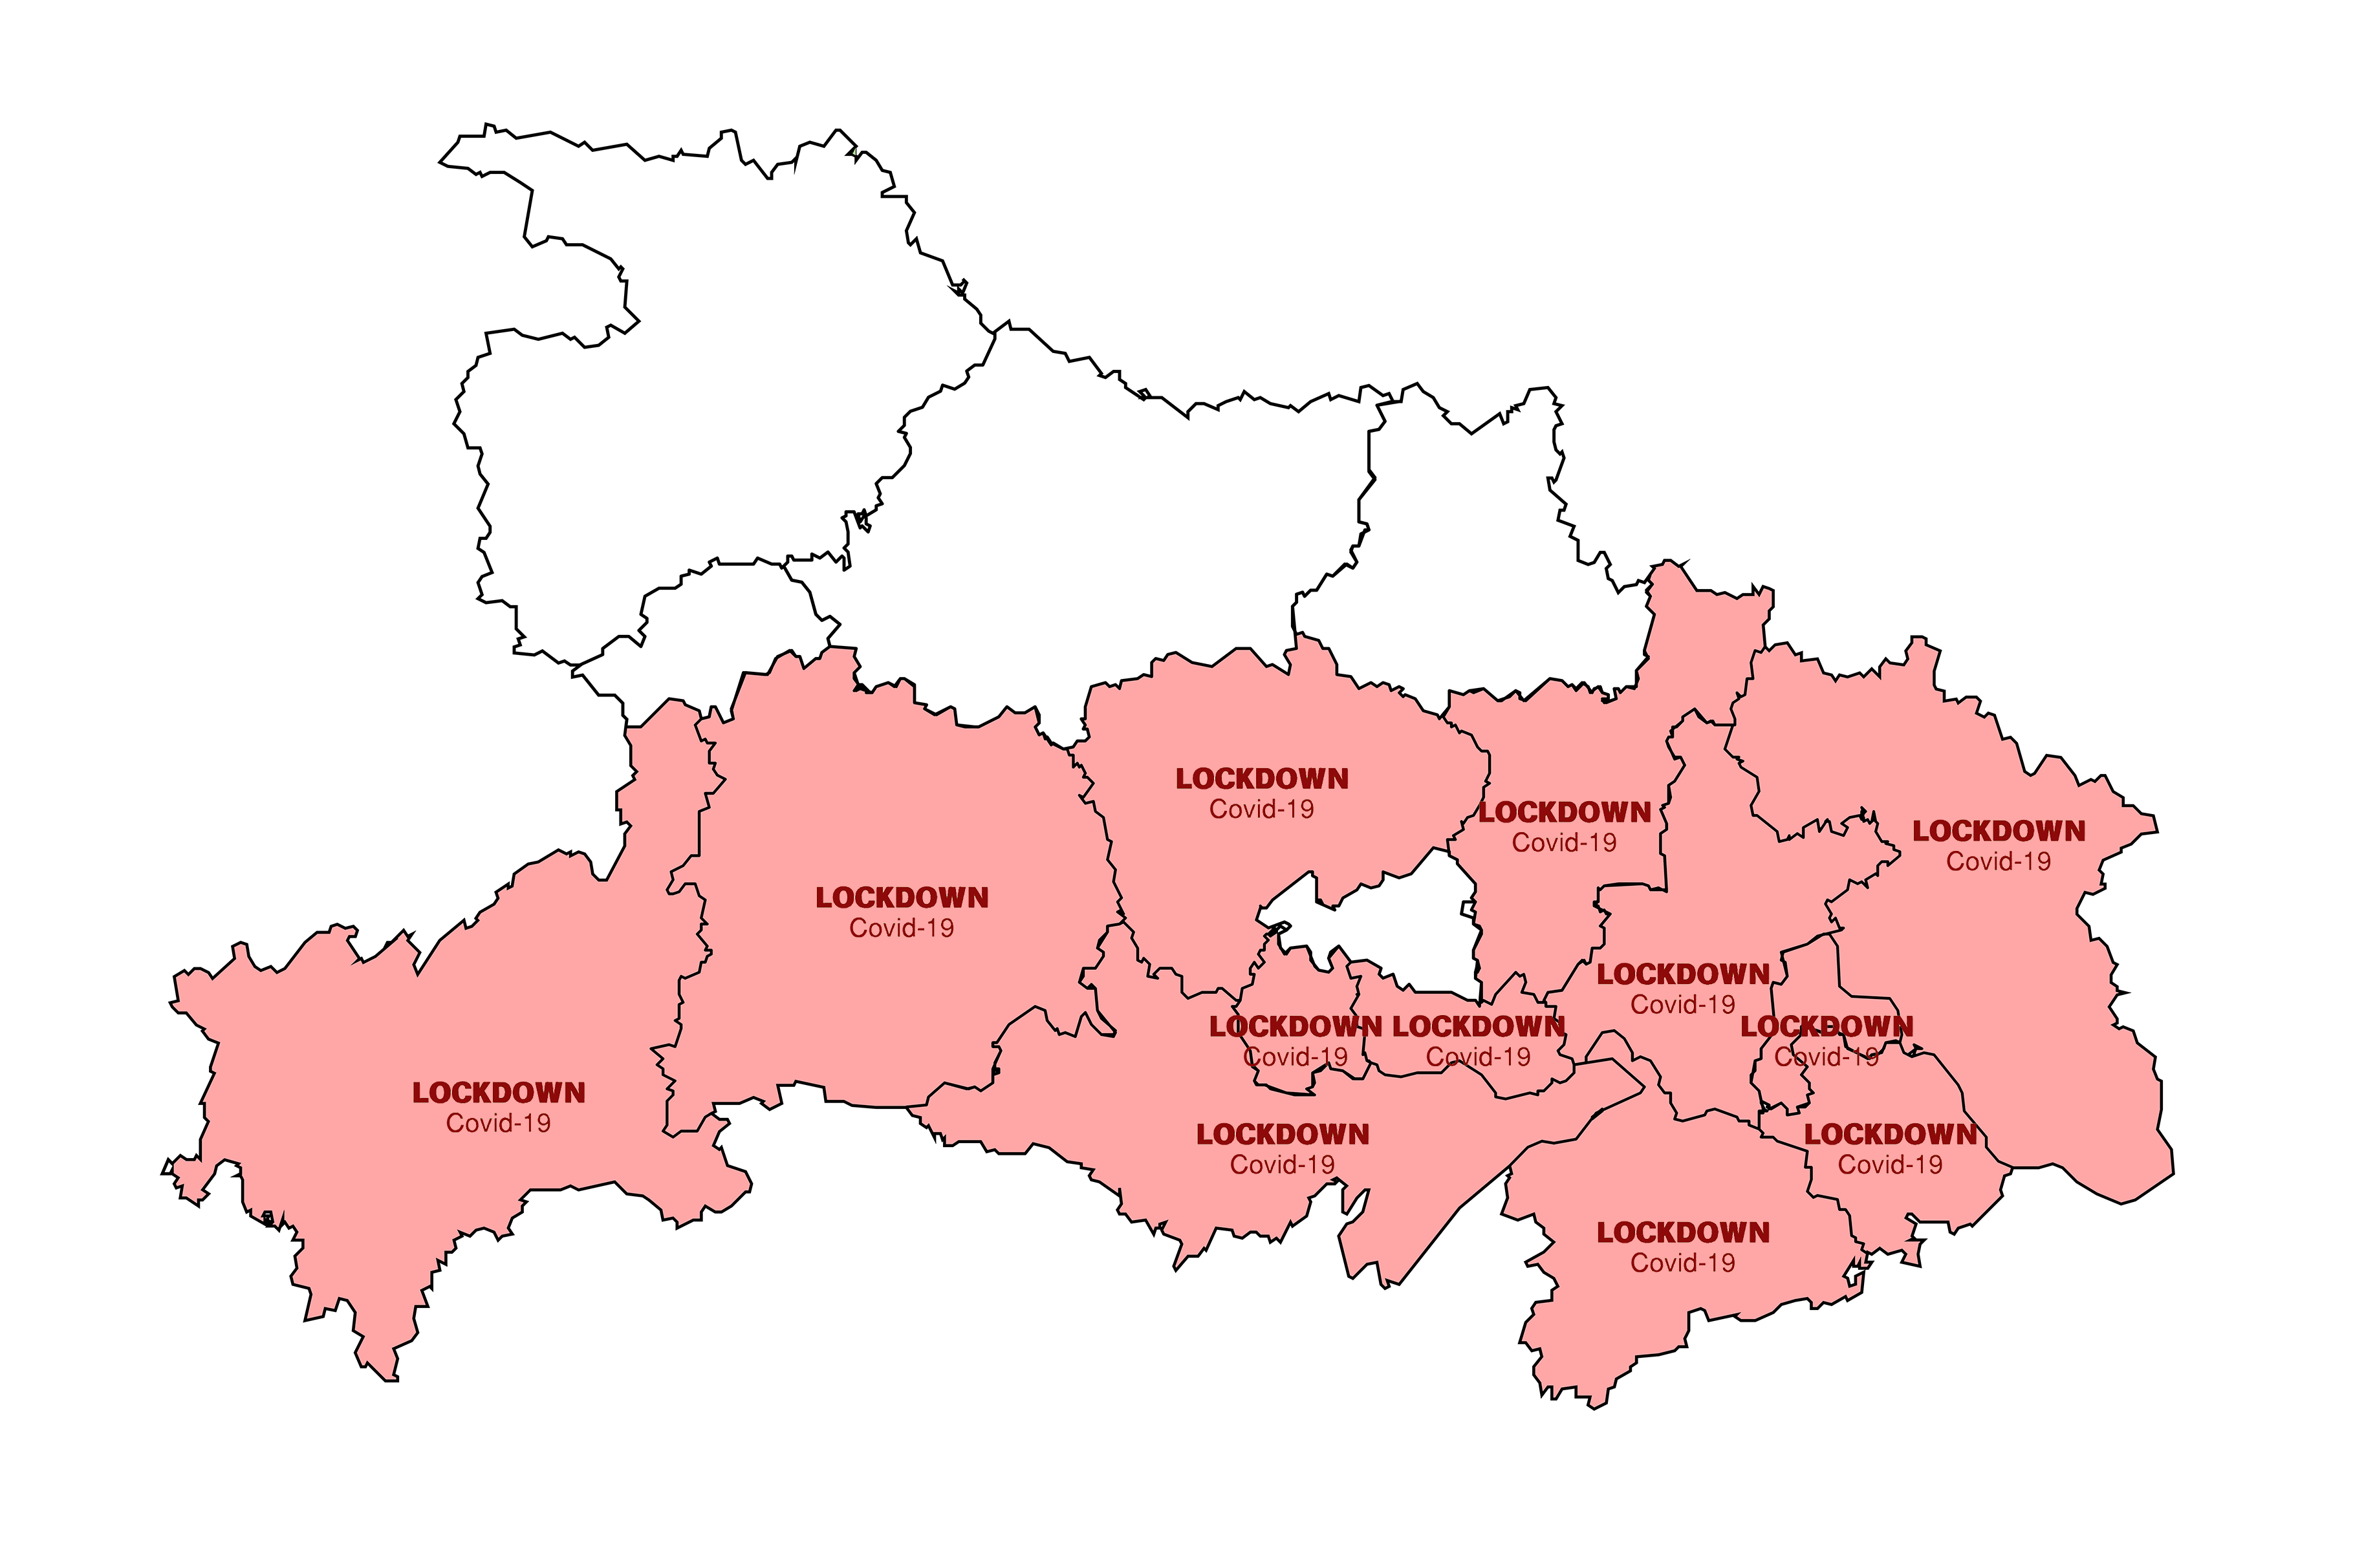
\includegraphics[width=\linewidth]{hubei.png}
    \caption{Map of the lockdown cities in the early stage of the outbreak, Hubei, China.}
\end{figure}

From the above statements, it is difficult to achieve precise and flexible epidemic prevention under the division of administrative regions.
We abandon the current epidemic control method based on administrative division and adopt a novel method which is based on GIS (Geographic Information System)\cite{clarke1986advances} and \textbf{GeoHash}.
\textbf{GeoHash} is a public domain geocode system invented in 2008 by Gustavo Niemeyer\cite{niemeyer2008geohash}.
\textbf{GeoHash} is used in GIS to divide the earth map into geometric blocks by encoding the the geographic locations into a short string of letters and digits.
The two-dimensional blocks are encoded by \textbf{GeoHash} bits, thus they are reduced to one dimension.
These blocks can be displayed as regular geometry (We take the grid shape as an example) on the map, and they can be scaled by the needs of observation scope change.

Our research finds that controlling epidemics based on blocks has the following advantages:
\begin{enumerate}
    \item The blocks divided by \textbf{GeoHash} are regular geometry, he shape can be customized by observer.
    \item The blocks are generated dynamically and they are scale-able according to the scope of infection.
    \item Information of the epidemic can be encoded in \textbf{GeoHash} or directly saved.
    \item The data in a block can be used to analyze through specific algorithms related to medical control.
    \item Users get epidemic information in their block in real time when such a GIS is released to the Internet.
\end{enumerate}

In the practical and experimental stage, we use mobile-application and web technology to implement such a GIS as shown in Fig. 2.
For medical staffs, it can work as an epidemic-related medical visual aid.
For ordinary users, it shares real-time analysis results and gives users safe travel suggestions.
\textbf{ASI} in Fig. 2 is a value of ``Area Safety Index'', which is the focus of our research.
It indicates the risk level of a region and will contribute to the decisions of governments, medical institutions, residents, and other researchers who are concerned about the epidemic.
\begin{figure}[h]
    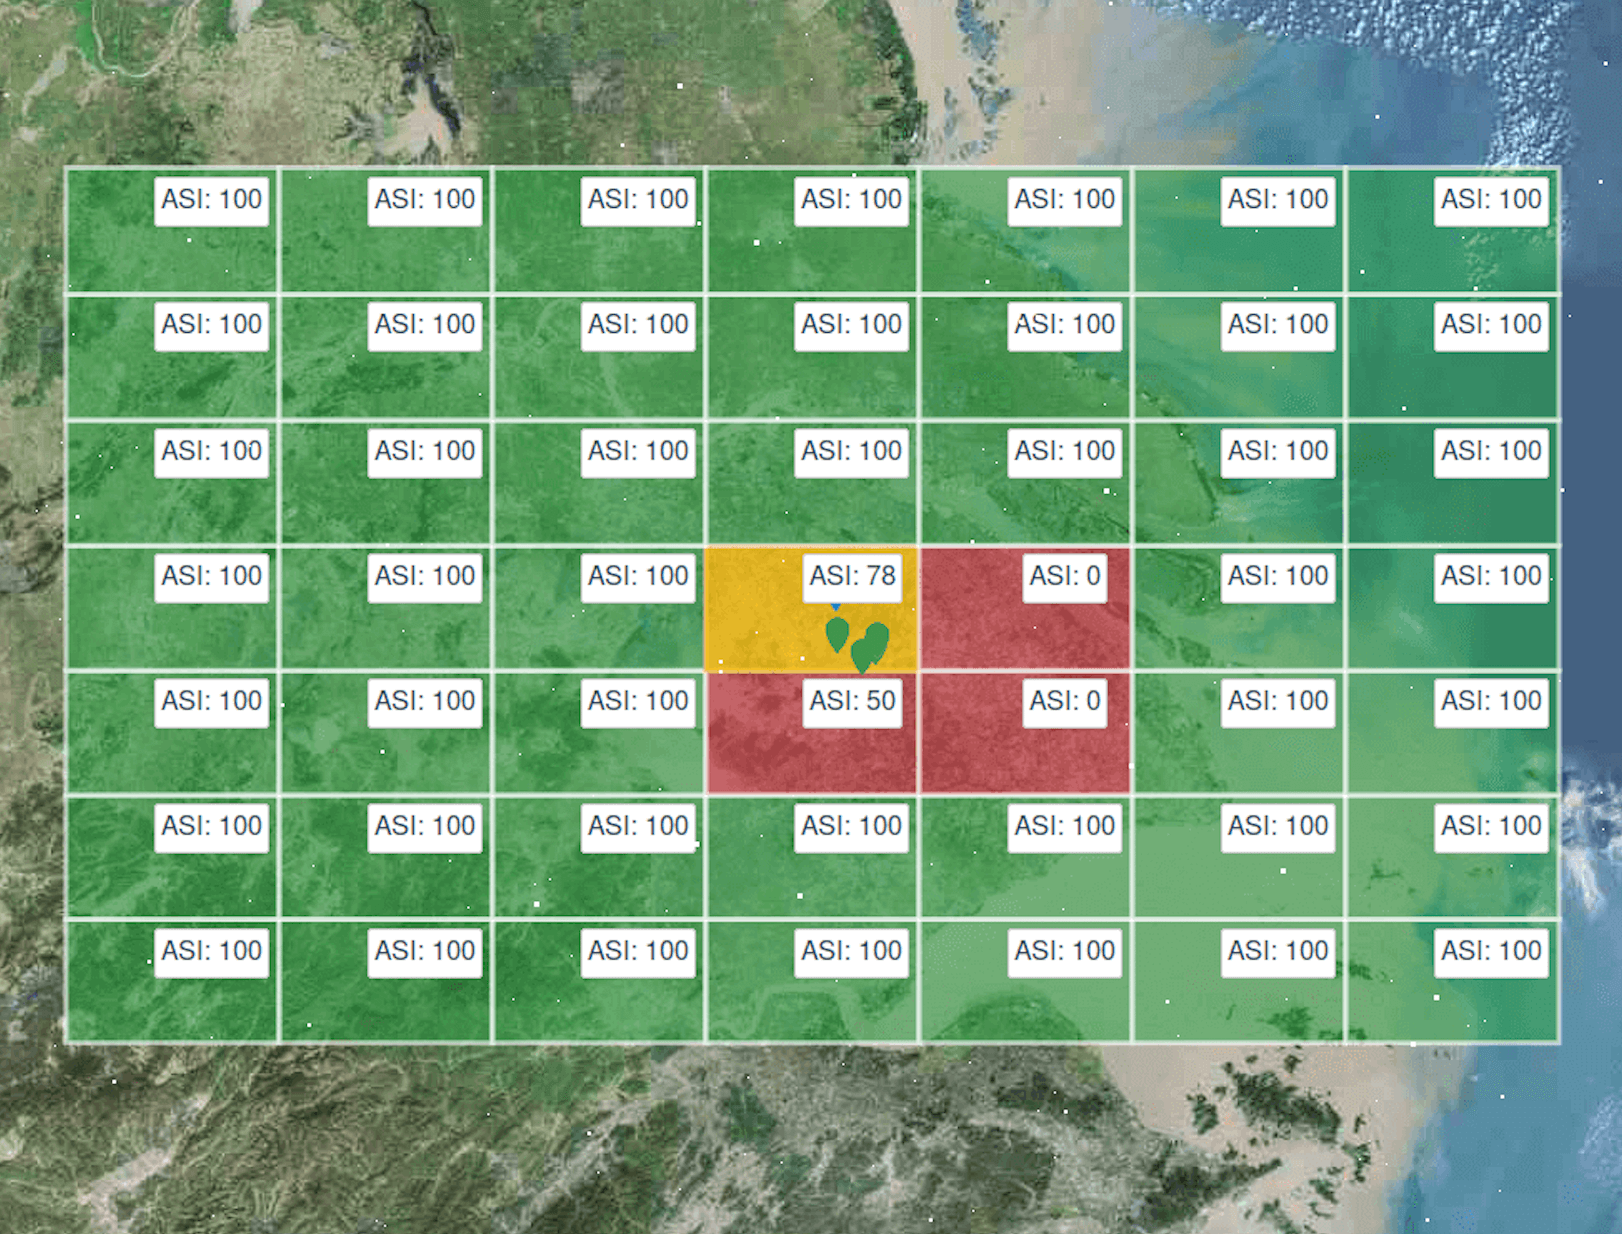
\includegraphics[width=\linewidth]{geogrids.png}
    \caption{Dynamic blocks divided by GeoHash in GIS}
\end{figure}

The core idea of our research is to divide the earth into several connected dynamic blocks (grids) and the blocks have the following characteristics:
\begin{enumerate}
    \item Blocks are regular geometry neighboring with each other.
    \item Blocks can be scaled on the map.
    \item Blocks are created only when they are meaningful.
    \item Scaling is limited, with the smallest and largest block size.
    \item Blocks can be scaled to discrete instead of continuous sizes.
    \item Structured data is stored in blocks, which can be used for data analysis.
\end{enumerate}

In the next section, we will also introduce other related work in controlling epidemic by using the information system and computer visualization technology.
Our research focuses on how to use \textbf{GeoHash} to divide the epidemic map and explains the methods of analyzing the epidemic-concerned data in \textbf{GeoHash} blocks.

\section{Related Work}
There are some mature cases of controlling and treating COVID-19 pandemic by using information systems and data visualization technology.
Many studies on COVID-19 have recently emerged, and various data science applications combating the pandemic have been reported recently\cite{latif2020leveraging}.
The main functions of these systems or software are listed as follows\cite{jia2020big}:
\begin{itemize}
    \item Tracking of people's movements.
    \item Early warning of high-risk areas.
    \item Screening of asymptomatic potential infections.
    \item Drug development.
    \item Information release and policy support.
\end{itemize}

\subsection{Data Visualization Analysis}
Visualization technology presents data to users by drawing charts and graphics, in which the data is represented by symbols, such as bar charts, line charts, pie charts, maps and etc \cite{jensen1992harvard}.
\begin{figure}[h]
    \centering
    \subfigure[Choropleth Map]{
        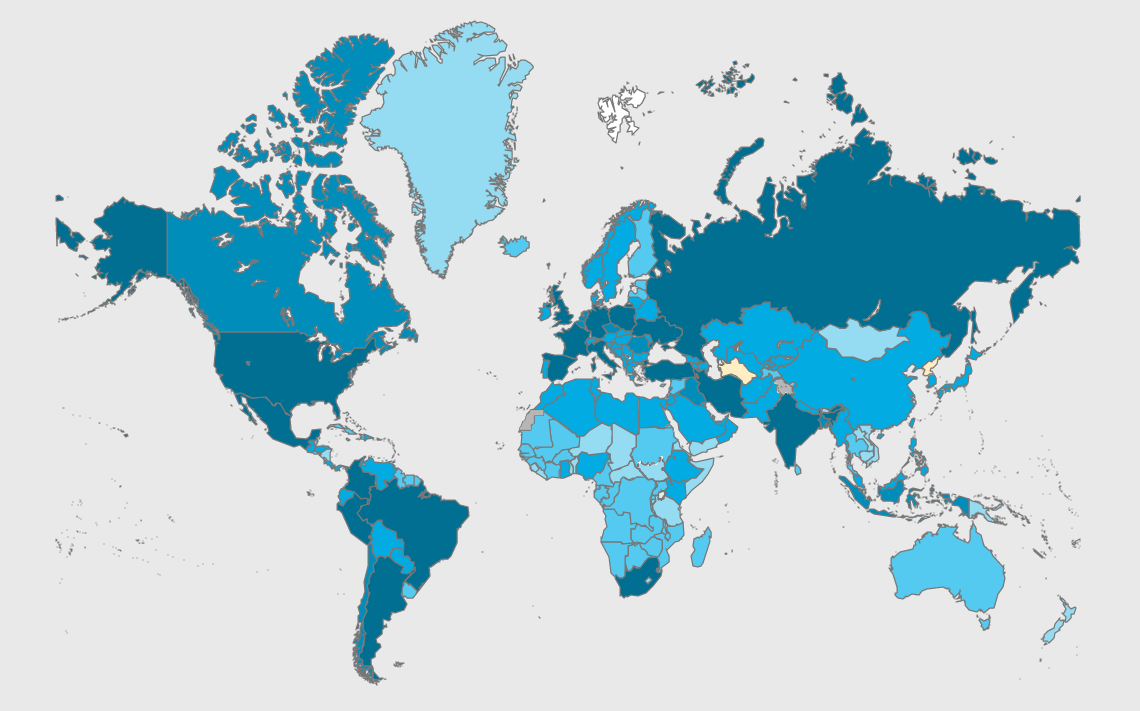
\includegraphics[width=0.95\linewidth]{worldmap1.png}
    }
    \subfigure[Bubble Map]{
        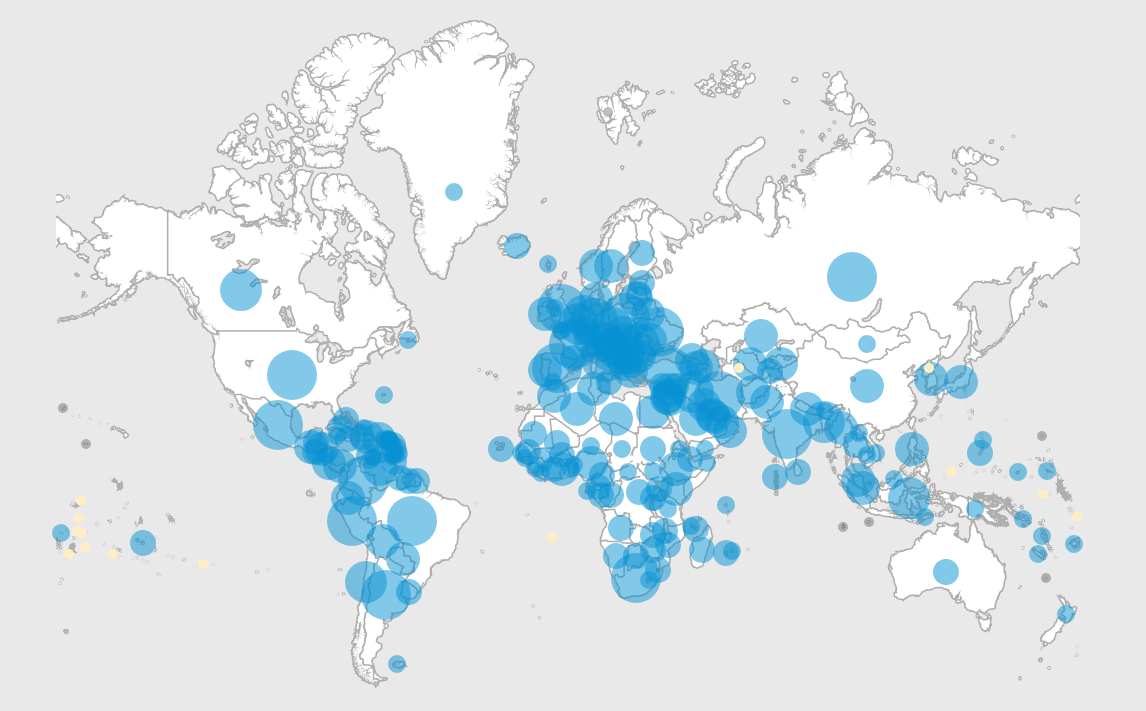
\includegraphics[width=0.95\linewidth]{worldmap2.png}
    }
    \caption{WHO coronavirus disease dashboard.}
\end{figure}

Fig. 3 shows the global COVID-19 epidemic situation in the form of map charts. The epidemic maps are updated by WHO (World Health Organization)\footnote{https://covid19.who.int} in real time, to display the number of cases around the world.

Maps in Fig. 3 uses two styles of presentation: (a) choropleth and (b) bubble.
Map (a) uses the depth of color to show the severity of the epidemic situation in each country, and (b) uses the bubble size to show the number of infections.
No matter which style of map it is, its role is to help human beings understand the severity of the epidemic easily, and prompt the local government to take actions to treat and control the epidemic situation.
The two maps in Fig. 3 are similar to the previous Fig. 1 of Hubei, except that Fig. 1 shows one province.
Contents in these maps include like: confirmed cases, deaths, historical cases, added cases, regional lockdown status, and etc.
Some weaknesses of such kind of maps have been discussed in the introduction section (Section \uppercase\expandafter{\romannumeral1}).
However, the data content contained in these maps gives us some enlightenment: what kind of data does a block need to contain?

Also, bar charts and line charts are widely used in epidemic data analysis.
They are mostly used to show the trend of epidemic situation and infection cycle.
Fig. 4 shows an example that uses both bar chart and line chart to perform the trend of daily new cases from Jan. 2020 to Jan. 2021 in the United States.
The red line in this chart is the 7-day moving average curve.
Other trends from different types of data, such as death trends, can be found on the official CDC\footnote{https://covid.cdc.gov/covid-data-tracker} website.
\begin{figure}[h]
    \centering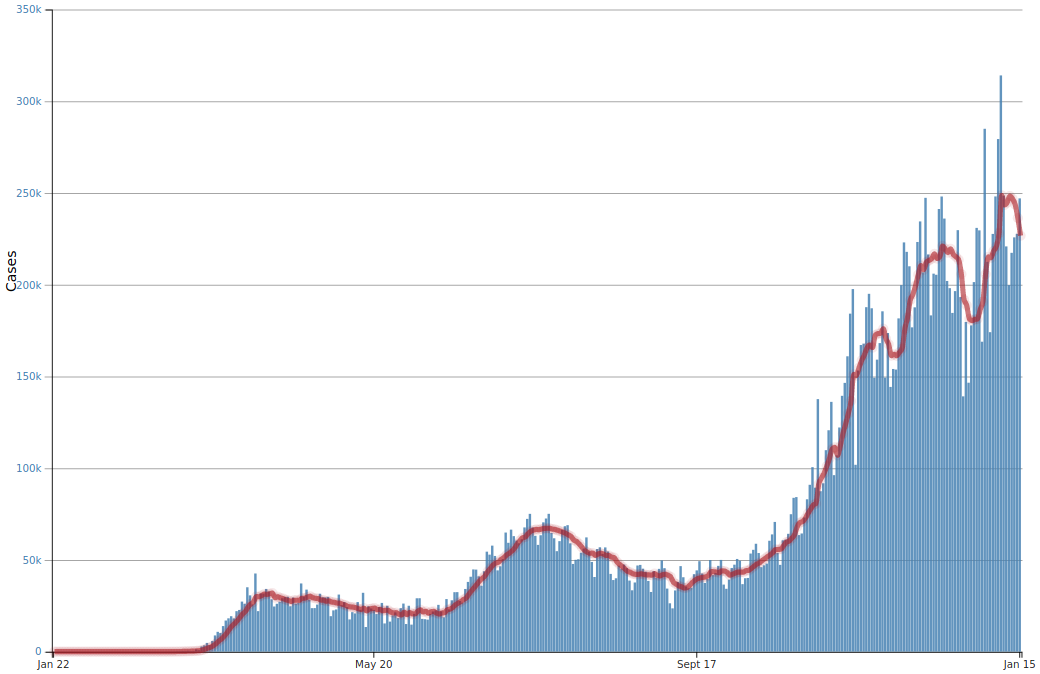
\includegraphics[width=\linewidth]{linebar-us-1-15.png}
    \caption{Daily trends in number of COVID-19 new cases in the US reported to CDC.}
\end{figure}

The line charts and bar charts reflect historical epidemic data from time series, while map charts reflect epidemic data from spatial distribution.
In other related work survey, visual data analysis are used to study the relationship between population mobility and the epidemic spreading pattern.
During the early outbreak of coronavirus in Wuhan, China, the graphs in a research suggested that the number of confirmed cases in other provinces were directly proportional to the inflow of Wuhan population.
The research group also used the pattern derived from the data analysis to predict the number of infections\cite{chen2020data}.

\subsection{Geographic Information System}
The maps we described in the previous section are charts, the information carried by map charts is limited, inflexible, without automatic analysis and not in real time.
Although charts can provide visual perception, users need to analyze the graphs by themselves, but GIS can integrate analysis, prediction and other practical and advanced functions.
A GIS is a conceptualized framework that provides the ability to capture and analyze spatial and geographic data\cite{clarke1986advances}.
Since the outbreak of the epidemic, a number of geographic information systems have been built or have added real-time epidemic related functions, such as ``epidemic map displays'', ``fever clinic queries'' and ``passenger information queries''.
Based on existing commercial GIS software, they made important contributions to epidemic prevention and control\cite{zhou2020covid}.
Some of the systems have the function of dynamic zoom map, which can display the situations of different scaling areas, from state level to community level.
For example, Fig. 5 shows a map with an epidemic layer on it, it is a GIS tool that shows critical information about COVID-19 cases in an area and users can make more informed decisions about where to go.
\begin{figure}[h]
    \centerline{
        \subfigure[State Level]{
            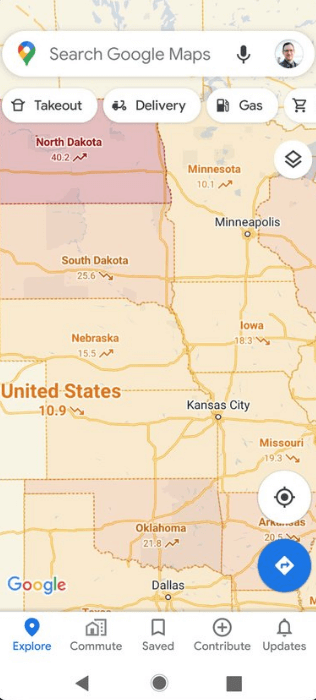
\includegraphics[width=0.48\linewidth]{state-level.png}
        }
        \subfigure[County Level]{
            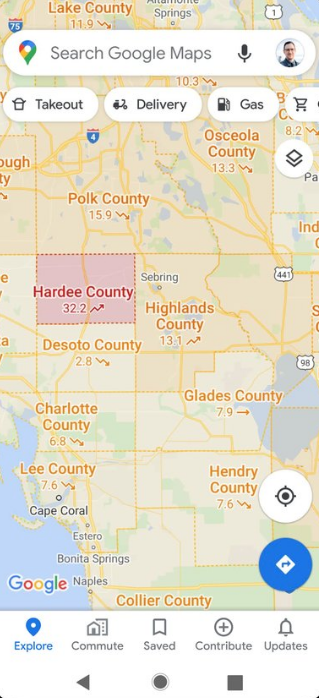
\includegraphics[width=0.48\linewidth]{county-level.png}
        }
    }
    \caption{COVID layer on Google Map on different scales}
\end{figure}

In Fig. 5, \textbf{Google Map} adds a COVID-19 layer to its GIS, it also quantities an safety index by using the 7-day average for the number of new cases per 100,000 people.
It also indicates whether cases are increasing or decreasing.
The layer's colors indicate:\footnote{https://support.google.com/maps/answer/9795160}
\begin{itemize}
    \item Grey: less than 1 case.
    \item Yellow: 1 to 10 cases.
    \item Orange: 10 to 20 cases.
    \item Dark orange: 20 to 30 cases.
    \item Red: 30 to 40 cases.
    \item Dark red: 40 more cases.
\end{itemize}

Unlike \textbf{Google Map}, we perform the quantitative analysis based on dynamic \textbf{GeoHash} blocks instead of administrative regions.
The safety quantification algorithm we use not only includes the simple infected cases.

\subsection{Precise Epidemic Prevention \& Control}
In this section, we will introduce research on precision epidemic prevention and control.
However, the approaches proposed in these studies are mainly related to data sharing and data analysis, without involving the computer visualization techniques.
A study conducts by\cite{cai2020demand} suggests that the precision of epidemic prevention and control can be effectively and comprehensively improved through the sharing of epidemiological data among medical institutions.
In this paper, a platform called ``one-net management'' is mentioned, which is established in Shanghai, China, to support dynamic information monitoring in this city.

More research comes from the medical field.
They focused on modeling the spread of the virus through existing epidemic data, such as\cite{small2020modelling}.
It proposes a detailed model of the topology of the contact network under various external control regimes and demonstrate that this is sufficient to capture the salient dynamical characteristics and to inform decisions.

In the following sections, we will focus on our research work about how to use \textbf{GeoHash} to improve the GIS for epidemic prevention and control.

\section{Methodology}
Our challenges are mainly from two aspects: data collection and data quantification.
Although data collection has been integrated into GIS, it requires the user to authorize GPS on the device to obtain and upload locations to our service.
Quantitative analysis of data is a more complex process and our work is to quantify the collected messy data in each \textbf{GeoHash} block.
\subsection{Data Preparation}
For data collection, our research provides a mobile application for our users to view the surrounding epidemic situation.
At the same time, in order to obtain the surrounding epidemic safety situation, users are required to share their GPS data.
Under the privacy policy, our application collects users' GPS information under their authorization only, and never collects users' personal information.
The method of GPS data collection is carried out anonymously, and each record is stored as a virtual and unknown user identity which means we know where the location is but never know whom the location belongs to.

After being confirmed, a medical staff needs to label the patient in a virtual identity.
A user can never know other users' real identities, but can browse surrounding infection with the locations of these cases.
Only the medical staff knows a patient's true identity to track the blocks the patient has visited.
Briefly speaking, our solution is to use a virtual identity or mask user's information to separate user location information and user personal information.
This is an approach to keep a balance between keeping user privacy and collecting data for epidemic control.
In fact, several similar approaches have been put into effect.
In China, a kind of QR code generated by a mobile application called \textbf{Health Code} displays one's health status but doesn't tell one's information.
Each \textbf{Health Code} corresponds to a real-name-certificated user.
In daily life, citizens use \textbf{Health Code} to know the health status of themselves or others.
In some public places, \textbf{Health Code} is required as a "pass" to the markets, schools, hospitals, government departments, etc.

For data quantification, firstly we need to divide the map into blocks by using \textbf{GeoHash}.
At the step of GPS data collection, we get the values of longitude and latitude from users.
\textbf{GeoHash} will calculate which block the user belongs to.
Suppose a \textbf{GeoHash} block as a set $B_1$ that includes many users $U_1, U_2, U_3\ldots$, we quantify the safety index of $B_1$ through the confirmed cases, suspected cases (close contacts), total cases it contains.
Also, the historical users, ``visitors'' in a block are needed to be considered.
These visitors who have been infected or closely contacted with those confirmed cases enter the block even in a short term and they also have negative effects on the block.

As discussed above (in Section \uppercase\expandafter{\romannumeral2}.A), research has proposed that the number of people infected in a region is positively correlated with the inflow of the population from high-risk areas.
That means, when collecting location data, we need to store not only a user's current location but also his or her historical location data.
The general process of user data storage and analysis is shown in Fig. 6.
\begin{figure}[h]
    \centering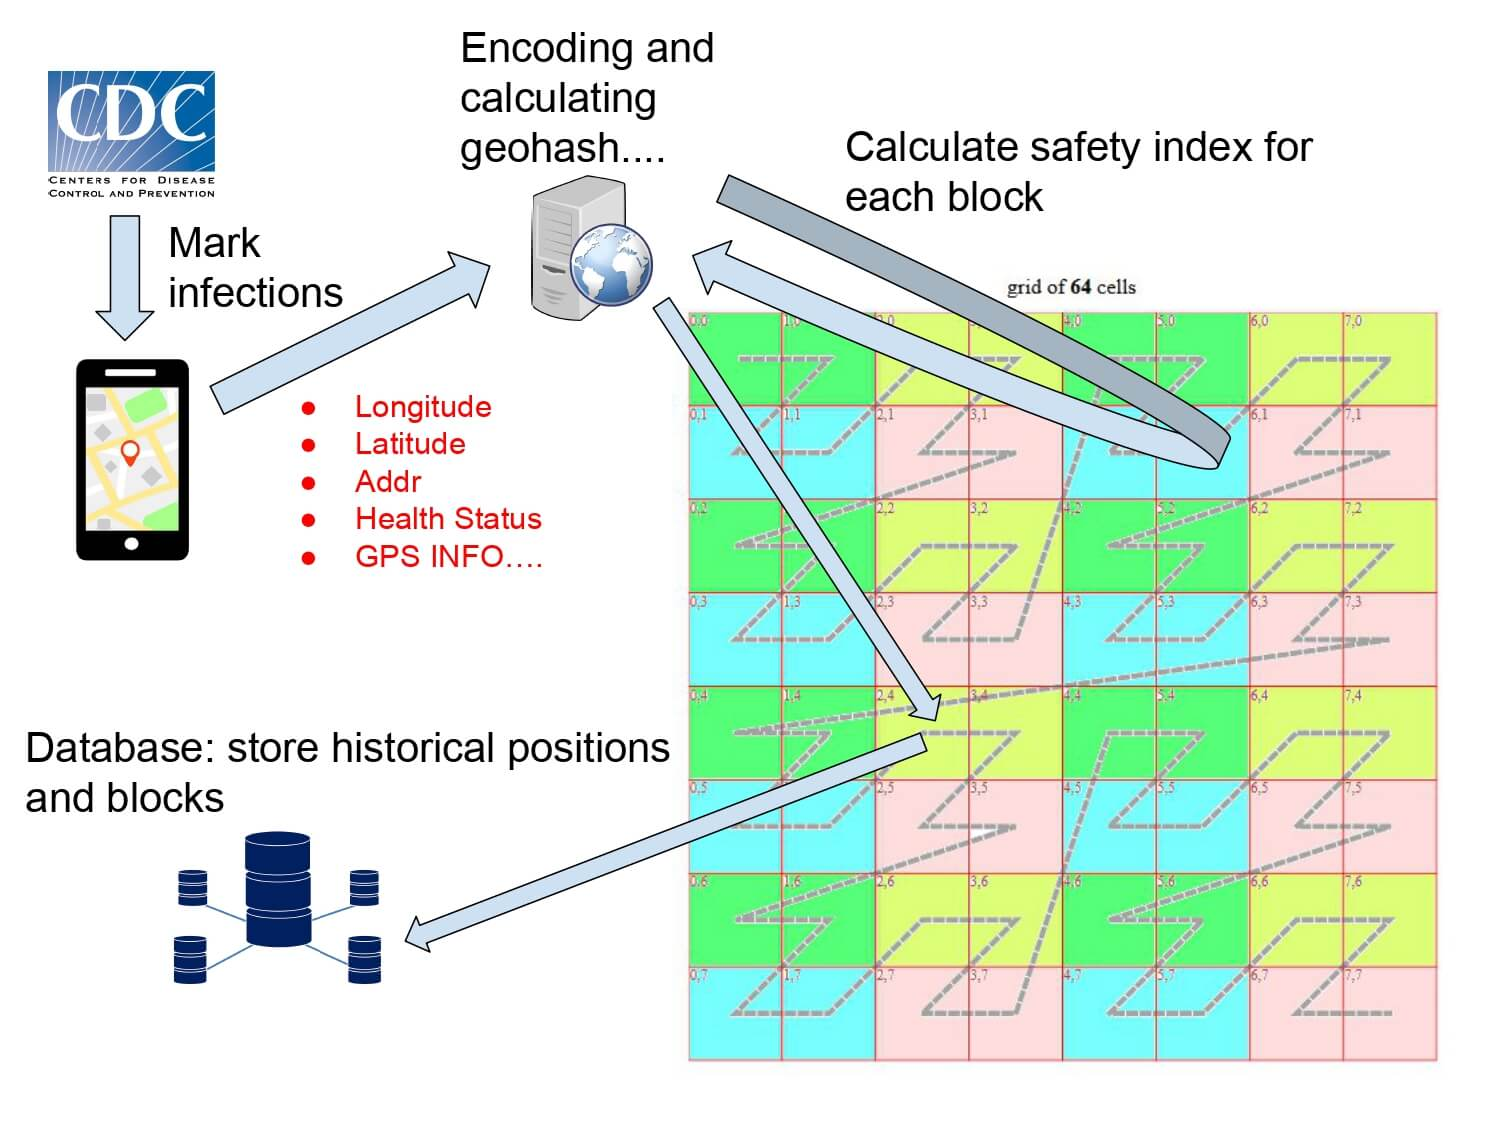
\includegraphics[width=\linewidth]{process.jpg}
    \caption{The process of data collection and quantification}
\end{figure}

Each row of data contains some necessary attributes: \textit{userid}, \textit{longitude} and \textit{latitude}, and \textit{\textbf{USI}}\footnote{USI is ``User Safety Index'', a value of user's health index in our model}.
Based on the above data, we can divide users into different blocks.
\subsection{Grid Division}
Our first step is to divide the earth into blocks or grids. \textbf{GeoHash} technology can help us achieve this step.
\textbf{GeoHash} can perform the following operations:
\begin{itemize}
    \item \textbf{GeoHash} divides a two-dimensional map into buckets of grid according to the range of longitude and latitude.
    \item \textbf{GeoHash} encodes a geographic location (longitude and latitude) into a string of binary codes.
    \item Through the incremental operation of encoded binary code, these grids are chained to a Z-order curve as Fig. 7.
\end{itemize}

How does \textbf{GeoHash} achieve the above operations?
We know that the geographical range of longitude is from $-180\degree$ to $180\degree$ and latitude is from $-90\degree$ to $90\degree$\cite{crossley1999guide}.
We can divide the longitude into two intervals: $[-180\degree, 0\degree]$, $[0\degree, 180\degree]$.
We denote the two intervals by binary number ``$0$'' and ``$1$'' respectively.
In an equivalent way, we divide the latitude into two intervals: $[-90\degree, 0\degree]$, $[0\degree, 90\degree]$ and denote them by ``$0$'' and ``$1$''.

Then we can use ``$00$'', ``$01$'', ``$10$'', ``$11$'' to represent the four grids.
Fig. 7 gives the examples of ``The earth is divided into 4 grids'' and ``The earth is divided into 16 grids''.
However, in this way, the area of each grid is quite large, and the grid precision is too low.
The same way is used to further subdivide into 16, 64 grids, etc.
We get higher precision by adding the bits of \textbf{GeoHash} binary which means the earth is divided into more and smaller grids.
\begin{figure}[h]
    \centerline{
        \subfigure[4 grids]{
            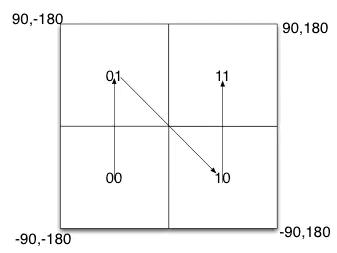
\includegraphics[width=0.48\linewidth,height=35mm]{4-grids.png}
        }
        \subfigure[16 grids]{
            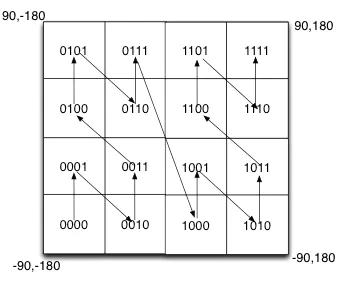
\includegraphics[width=0.48\linewidth,height=35mm]{16-grids.png}
        }
    }
    \caption{Z-order curve to show \textbf{GeoHash} grids division}
\end{figure}

\subsection{Gird Size}
Table 1 compares the real-world geographical distance and the length of \textbf{GeoHash} bits, the latitude is around $30\degree$.
\begin{table}[h]
    \centering
    \caption{Comparison table of \textbf{GeoHash} bits and estimated geographical length of one grid}
    \begin{tabular}{llc}
        \toprule
        East-West Length(m) & South-North Length(m) & Bits \\
        \midrule
        32.67               & 19.05                 & 20*2 \\
        65.34               & 38.1                  & 19*2 \\
        130.68              & 76.2                  & 18*2 \\
        261.36              & 152.4                 & 17*2 \\
        522.72              & 304.8                 & 16*2 \\
        1045.44             & 609.6                 & 15*2 \\
        2090.88             & 1219.2                & 14*2 \\
        4181.76             & 2438.4                & 13*2 \\
        8363.52             & 4876.8                & 12*2 \\
        16727.04            & 9753.6                & 11*2 \\
        33454.08            & 19507.2               & 10*2 \\
        66908.16            & 39014.4               & 9*2  \\
        133816.32           & 78028.8               & 8*2  \\
        267632.64           & 156057.6              & 7*2  \\
        535265.28           & 312115.2              & 6*2  \\
        1070530.56          & 624230.4              & 5*2  \\
        2141061.12          & 1248460.8             & 4*2  \\
        4282122.24          & 2496921.6             & 3*2  \\
        8564244.48          & 4993843.2             & 2*2  \\
        17128488.96         & 9987686.4             & 1*2  \\
        \bottomrule
    \end{tabular}
\end{table}

Since the geometric shape of the earth is a sphere, even with the same \textbf{GeoHash} bits length, the grids of high latitude contain less geographical length than those of low latitude.
Attention: the length data in Table 1 is generated from the grids around $30\degree$ latitude, it doesn't represent all the grids or an average value.

We use the following formulas (1) and (2) to estimate the length of the two edges of one grid and it assumes the earth is completely spherical.
We use $G_{NS}$ to represent the length of north-south edge and $G_{EW}$ to represent the length of east-west edge as they are stroked in Fig. 8.
The power $geobit$ is the length of the \textbf{GeoHash} bits that are needed to represent a grid.
The length of a meridian which is $L_{meridian}$ in Formula (1) has been estimated at $20,003.93$ km ($12,429.9$ miles) on a modern ellipsoid model of the earth (WGS 84)\cite{weintrit2013so}.
The length of the equator which is $L_{equator}$ in Formula (2) is about $40,075$ km ($24,901$ miles)\cite{equator2011}.
Formula (1) is used to estimate the length of the north-south edge of a grid.
Formula (2) is used to estimate the length of the east-west edge of a grid at latitude $\varphi$.

\begin{equation}
    G_{NS}\approx\frac{L_{meridian}}{2^{geobit/2}}
\end{equation}
\begin{equation}
    G_{EW}(\varphi)\approx\frac{L_{equator}\times\cos(\varphi)}{2^{geobit/2}}
\end{equation}

\begin{figure}[h]
    \centering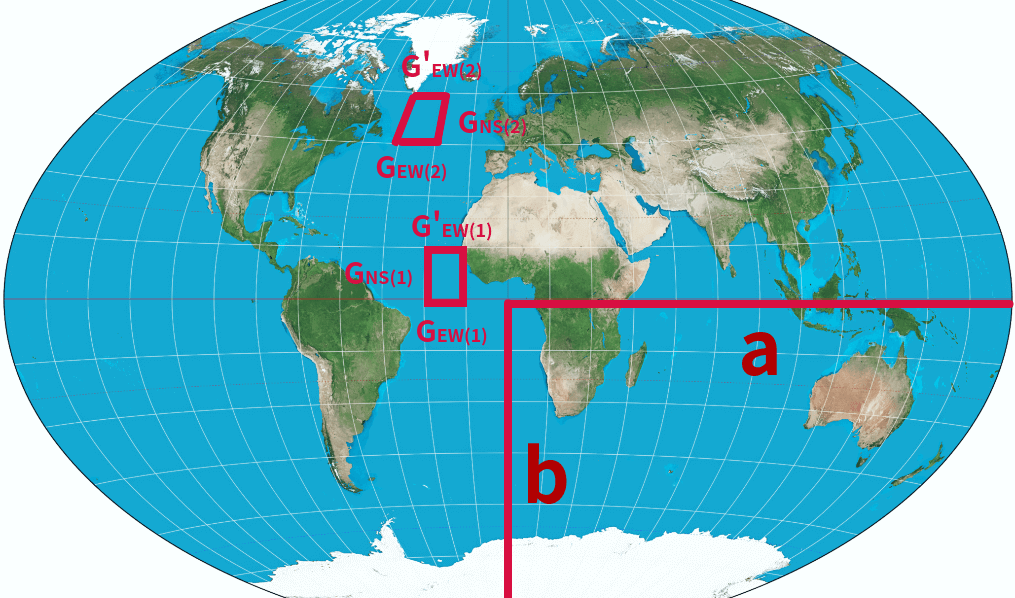
\includegraphics[width=\linewidth]{earth.png}
    \caption{Grid of elliptical earth}
\end{figure}

The reason why the word ``estimate'' is used when calculating $G_{NS}$ and $G_{EW}$ is that the earth is actually elliptical.
The ellipsoid earth will cause the following two issues:
\begin{itemize}
    \item The meridian and equator are different in length, grids at different latitudes own different $G_{NS}$ values.
    \item A grid is not a rectangle, two different $G_{EW}$ values will appear in one grid.
\end{itemize}

In fact, under the same \textbf{GeoHash} bits, whether it is ``Earth Ellipsoid'' or ``Earth Spheroid'', the length of the two edges of a grid depends only on latitude.
If we need a more precise length of the two edges, we should start a deep discussion about ``length of a degree of longitude'' and ``length of a degree of latitude'' which is beyond our research topic.
Here we list our final calculation formulas when the earth is modelled by an ellipsoid, this is much more complicated but exact than the spherical earth.

\begin{equation}
    a=\frac{L_{equator}}{2\pi}\quad
    b=\frac{L_{meridian}}{2\pi}
\end{equation}
\begin{equation}
    f=\frac{a-b}{a}\quad
    e^2=f(2-f)
\end{equation}
\begin{equation}
    \bigtriangleup\varphi=\frac{180}{2^{geobit/2}}
\end{equation}
\begin{equation}
    G_{EW}(k)=\frac{2\pi a\cos(k\Delta\varphi)}{2^{geobit/2}\sqrt{1-e^2\sin^2k\Delta\varphi}}
\end{equation}
\begin{equation}
    G_{NS}(k)=a(1-e^2)\int_{k\Delta\varphi}^{(k+1)\Delta\varphi}\frac{d\phi}{{(1-e^2\sin^2\phi)}^\frac32}
\end{equation}
\begin{equation}
    k\in\{-2^{\frac{geobit}{2}-1}, -2^{\frac{geobit}{2}-1}+1,\ldots, 2^{\frac{geobit}{2}-1}-1\}
\end{equation}

Formula (3), (4), (5), (6), (7) and (8), give the methods to estimate the grid size of the elliptical earth.
They are used to calculate the each side length of a grid.
The formulas are derived and modified from \textit{The Mercator Projections}\cite{osborne2013mercator}.
Each \textbf{GeoHash} grid in our GIS has 3 different side lengths, and they are represented by $G_{NS}(k)$, $G_{EW}(k)$ and $G_{EW}(k+1)$ respectively.

\subsection{Block Storage}
We store both the block information and user data, including:
\begin{enumerate}
    \item User historical location data
    \item Block data
\end{enumerate}

One block contains many users, and one user has many historical locations.
The information of block and user are bidirectionally associated which is called “many to many” in the field of computer data storage model.
This section will discuss the data storage models and algorithms.

Before storing the block, we have to encode the location by \textbf{GeoHash}.
The first step is to transform longitude and latitude to binary code.
Referring to the description about grid division in Section \uppercase\expandafter{\romannumeral3}.B, we adopt Algorithm 1.

\begin{algorithm}[h]
    \caption{Transform location to GeoHash bit}
    \begin{algorithmic}[1]
        \Require{$longitude,latitude,bit$, bit is the length of GeoHash}
        \Ensure{Integer array, GeoHash binary code}
        \Function{geohash}{$longitude,latitude,bit$}
        \State{$result=[]$}
        \State{$i=0$}
        \State{$lat[0]=-90$}
        \State{$lat[1]=90$}
        \State{$lon[0]=-180$}
        \State{$lon[1]=180$}
        \While{$i<bit*2$}
        \State{$mid=(lon[0]+lon[1])/2$}
        \If{$mid>longitude$}
        \State{$result[i++]=0$}
        \State{$lon[1]=mid$}
        \Else
        \State{$result[i++]=1$}
        \State{$lon[0]=mid$}
        \EndIf
        \State{$mid=(lat[0]+lat[1])/2$}
        \If{$mid>latitude$}
        \State{$result[i++]=0$}
        \State{$lat[1]=mid$}
        \Else
        \State{$result[i++]=1$}
        \State{$lat[0]=mid$}
        \EndIf
        \EndWhile
        \State{\Return{$result$}}
        \EndFunction
    \end{algorithmic}
\end{algorithm}

We have discussed that a \textbf{GeoHash} binary code can be divided into two parts: longitude part and latitude part, and they have the same length of bits in a \textbf{GeoHash} binary code.
In Algorithm 1, longitude and latitude are ranked one by one.
For example: in a returned \textbf{GeoHash} binary code, the first bit represents the range of longitude, then the second bit represents the range of latitude, and the third bit is longitude again, and so on.
This is a way for code simplicity, and theoretically, how to sort \textbf{GeoHash} binary bits is not disputed as long as the encoding and decoding rules are consistent.

If we directly store the \textbf{GeoHash} binary code of a block, a string of binary code is too long.
For more convenient access to these \textbf{GeoHash} blocks, we convert those binary code to hexadecimal string and store the ``hex code'' in a non-relational database.
Therefore, a string of hex code can represent a \textbf{GeoHash} block as well as a series of locations.
Fig. 9 shows a complete process of ``From location to \textbf{GeoHash} hex code''.

When a location needs to be determined, hexadecimal code can be easily converted to binary code, and then the binary code can be decoded to the range of longitude and latitude by inversing the \textbf{GeoHash} algorithm.
The accuracy of restored location depends on the original number of \textbf{GeoHash} bits.
In the research, we choose 10 to 20 bits \textbf{GeoHash} to encode longitude and latitude respectively, so the total length of a generated \textbf{GeoHash} binary is 20 to 40 bits.
In the experiment, we consider such sizes of blocks are the most reasonable observation range for medical workers.
Due to the flexibility of the algorithm, we can adjust the accuracy represented by each block as needed.

Fig. 9 has illustrated the data structure in the non-relational database.
\textbf{HashMap} is used to map between strings of keys and values.
We set user IDs as keys and user health information as values in a hash table.
In storage, one block corresponds to one hash table which contains multiple \textbf{HashMaps} and the hexadecimal code of a block is used as the name of a hash table.

When a user enters a block, the ID and information as a ``key-value'' pair will be recorded in a hash table.
When a user changes the location and enters another block, the user will be moved out of the current hash table and then be moved to the hash table of the new block.
\begin{figure}[h]
    \centering
    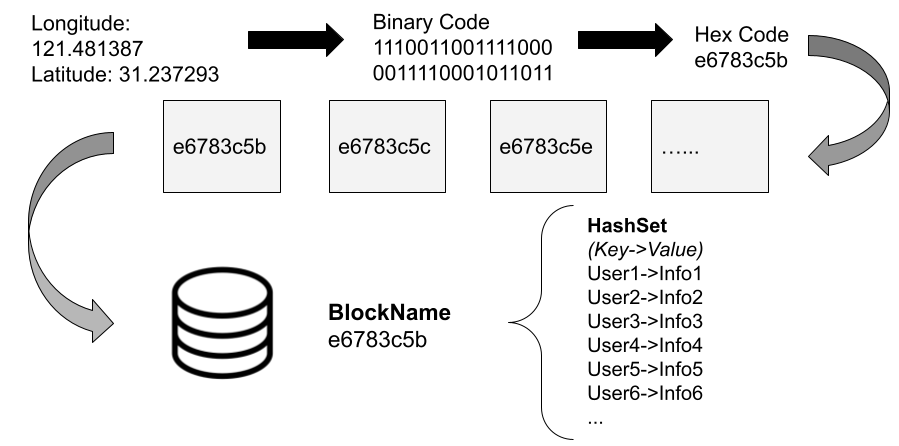
\includegraphics[width=\linewidth]{block-storage.png}
    \caption{The process of block storage}
\end{figure}
% 2020-5-25编辑至此

For those blocks that there is no user in it, we call them ``Depopulated Blocks''.
These blocks must be existed theoretically, such as the areas where the sea, mountains and the tropical rain forest is located.
In order to reduce the complexity of storage space, we should avoid recording these ``Depopulated Blocks''.
In contrast, when a user appears in a depopulated block, a new block will be created dynamically in the storage space, which means a new related hash table will be generated in the database, and the user's information will be recorded in it.

For those blocks that a user has accessed, they can be logged as another data structure \textbf{UGBL}.
In Fig. 10, blocks are stored as nodes in a link or an array data structure by following a head (user).
We call them ``User GeoHash Block Link'', \textbf{UGBL} for short.
The \textbf{GeoHash} blocks have been accessed by one user are sequentially pushed into the link and a user's ID is set as the head of the \textbf{UGBL} link.
The blocks that the user entered earlier will be placed at the tail of the link.
\begin{figure}[h]
    \centering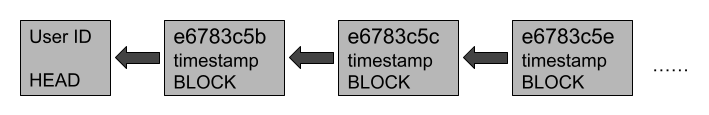
\includegraphics[width=\linewidth]{UGBL.png}
    \caption{User GeoHash Block Link data structure}
\end{figure}

COVID-19 requires us to query the past 14-days records which will generate a 14-days (15 nodes with one head and 14 blocks) \textbf{UGBL}.
It is worth noting that COVID-19 14-days \textbf{UGBL} data entities will be used in the next section for risk quantitative analysis of \textbf{GeoHash} blocks.

\subsection{Block Quantification}
For quantitative analysis of a block, the data that we need to use includes the current data and the past $n$ days' historical data of a block.
The ``14 days'' is for the example of COVID-19 because studies have shown that the longest incubation period of the virus is 14 days\cite{lauer2020incubation}.

The sample of quantitative analysis in our research is to obtain a value of \textbf{ASI} (Area Safety Index).
\textbf{ASI} is one of the most important indexes in our research, which reflects the safety degree of a \textbf{GeoHash} block.
The safety degree can be calculated to a meaningful and definite quantity with \textbf{ASI}.
The following is an introduction about calculating \textbf{ASI} of a block.
The following method is considered as our ``Basic ASI Model''
\begin{equation}
    RI_n=\sum_{i=1}^n\left(\frac{R_d^iP_d}{R_o^i+R_w^i+R_d^i}+\frac{R_w^iP_w}{R_o^i+R_w^i+R_d^i}\right)P_i
\end{equation}
\begin{equation}
    ASI_{cov19}=100-RI_{14}
\end{equation}
In Formula (9), $RI_n$ (Risk Index) represents the past $n$ days risk index of a block.
$R_d$, $R_w$ and $R_o$ are respectively the number of confirmed cases, suspected cases, and healthy cases.
So Formula (9) actually is a risk assessment by calculating the density of infected and suspected cases in a block.
Suspected cases refer to those who have symptoms of infection, have been in closely contact with confirmed cases, or have accessed high-risk blocks.
We define the blocks with \textbf{ASI} less than 60 as high-risk blocks, and the standard of high-risk can be customized in our model.
Variable $i$ counts the backtracking days.
For example, ``$i=n$'' indicates today, ``$i=n-1$'' indicates yesterday, until ``$i=1$'' is the first backtracking day, the total is $n$ days.
$P_d$ is the weight of infected cases and $P_w$ is the weight of suspected cases.
$P_i$ is the weight of time influence, the unit of time is ``day''.
Normally, the larger the day $i$ is, the higher the $P_i$ is.

Constants $P_d$ and $P_w$ can be dynamically adjusted according to the population in a block.
The calculation of $P_i$ is as Formula (11):
\begin{equation}
    P_i=\frac{100i}{(n+1)n/2}
\end{equation}

The time weight $P_i$ increase linearly with the increase of day $i$.
$n$ is a constant and it is the number of backtracking days in \textbf{ASI} calculation.

\section{Experiments}
Two groups of experiments are carried out on the block with large population and the block with small population.
The collective conditions of the two experiments for calculating \textbf{ASI} are:
\begin{enumerate}
    \item Simulate confirmed cases, suspected cases within 42 days.
    \item The backtracking time is 14 days, so $n=14$.
    \item If the backtrackable time is less than 14 days, set $n=i$.
    \item The total population in a block fluctuates up and down within a range.
    \item Upon \textbf{ASI} decreases to 60, the block will trigger lockdown, the population stops flowing in or out.
\end{enumerate}

We use \textbf{Apache Echarts}\footnote{https://echarts.apache.org/examples/en/editor.html?c=mix-line-bar} to visualize the experimental results.
In Fig. 11, the red line is a lockdown warning line, which also means that it is a high-risk state below this line.
The yellow line represents the trend of \textbf{ASI}.
The blue bar indicates the number of confirmed cases and the green bar indicates the number of suspected cases.
Both of the confirmed and suspected cases increase from day 1, and decrease after reaching the peak until 0.
\begin{figure}[h]
    \centering
    \subfigure[Small population]{ 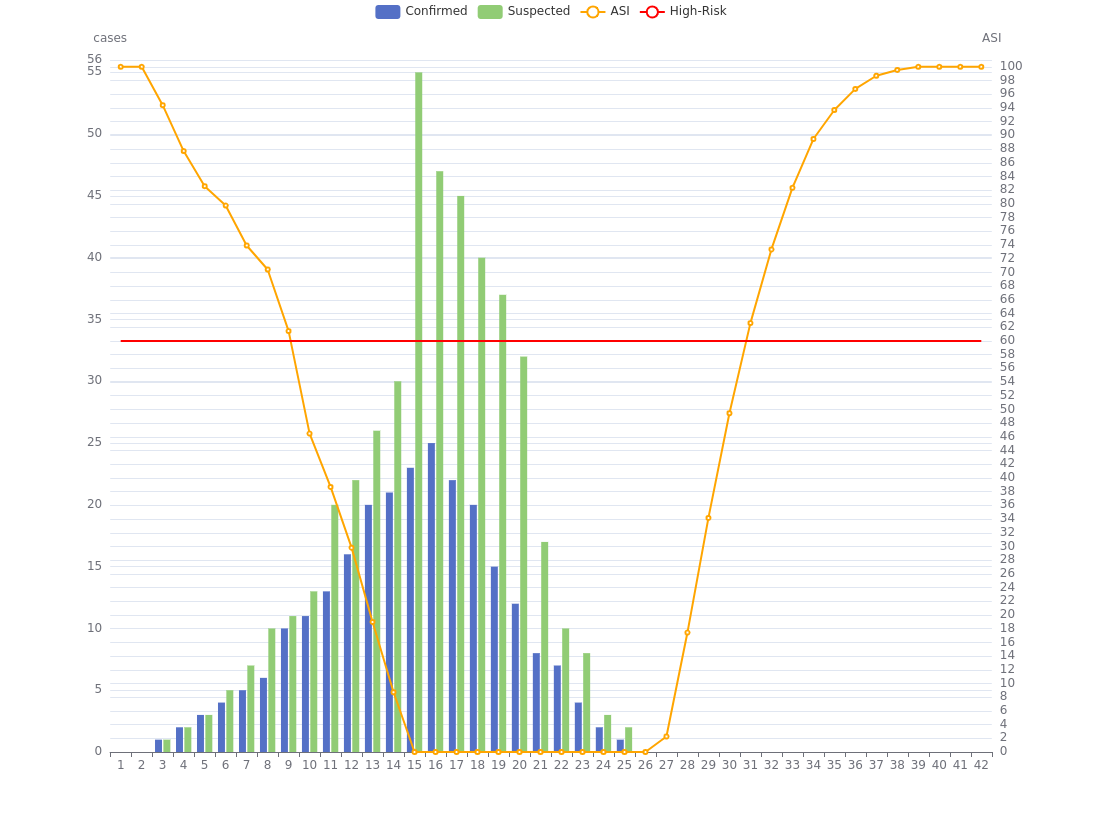
\includegraphics[width=0.95\linewidth]{echarts-sm.png} }
    \subfigure[Large population]{ 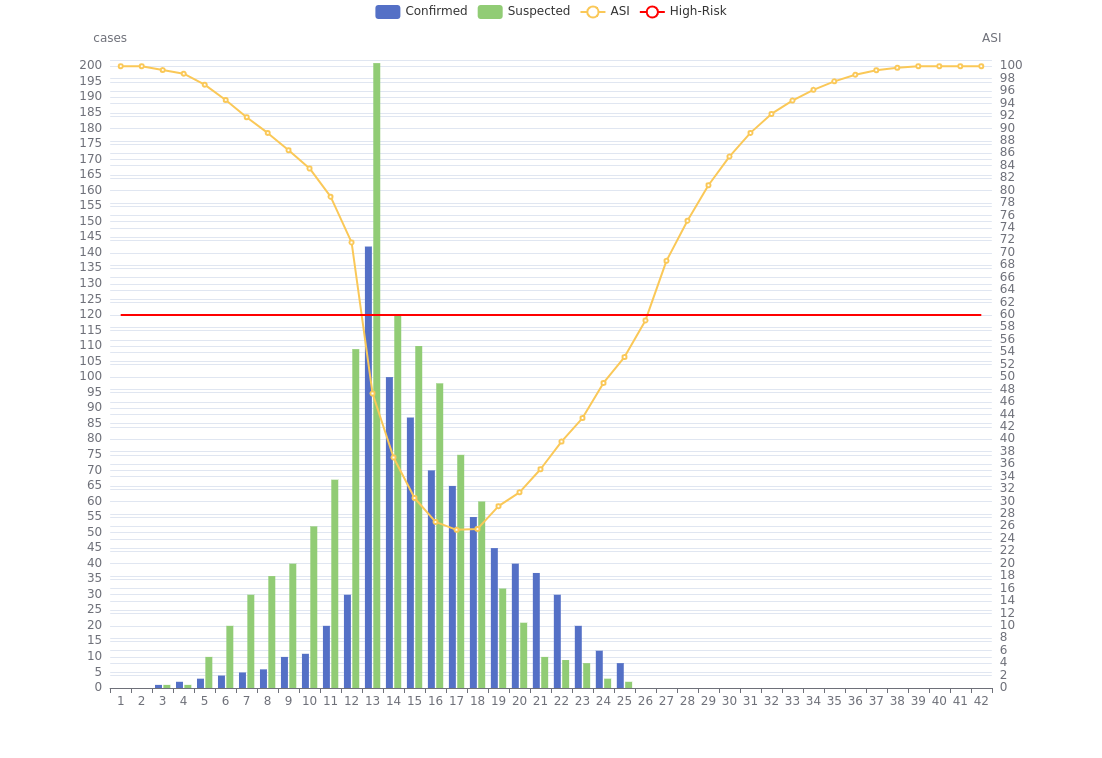
\includegraphics[width=0.95\linewidth]{echarts-lg.png} }
    \caption{The experimental results}
\end{figure}

\subsection{Small Population}
For a small population block, we assume the following conditions:
\begin{enumerate}
    \item The population range is $[500,1000]$ in a block.
    \item $P_d=45$ and $P_w=15$.
\end{enumerate}
The experimental results of small population block have been plotted as shown in Fig. 11, ``Small population''.
When the confirmed cases and suspected cases increase, \textbf{ASI} decreases.
\textbf{ASI} decreases to $46.47$ on day $10$ and drops to $0$ on day $15$.
Until day $31$, \textbf{ASI} returns to above $60$.
So we can set the block in high-risk from day $10$ to $31$.

\subsection{Large Population}
For a large population block, we assume the following conditions:
\begin{enumerate}
    \item The population range is $[960000,1000000]$ in a block.
    \item $P_d=8000$ and $P_w=4000$.
\end{enumerate}
The experimental results of large population block have been plotted as shown in Fig. 11, ``Large population''.
From the ``Large population'' chart, \textbf{ASI} decreases to $47.35$ on day $13$ and goes back to $68$ on day $27$.
Then we set the block in high-risk from day $13$ to $27$.

\section{Conclusions}
Based on \textbf{GeoHash}, we study a novel method to control the COVID-19 epidemic by dynamically encoding and dividing blocks from geographic locations.
In our research project, the dynamic storage, display and scaling of blocks on a GIS map are implemented.
Blocks can work without administraion and they are automatically generated by \textbf{GeoHash} algorithm and automatically covered on GIS through computer softwares.
According to the population, cases in each block, the \textbf{ASI} was obtained by quantitative analysis algorithm.
\textbf{ASI} can effectively support medical work, and also provide users with safe travel suggestions.
Finally, taking COVID-19 epidemic as an example, through two groups of experiments, we test the large population and small population blocks to ensure the reliability of \textbf{ASI} algorithm.
When \textbf{ASI} is lower than 60, we consider it is necessary to take lockdown or other effective measures of the block.

\section{Future Work}
In addition to \textbf{ASI}, we will also conduct other types of attributes and features data analysis on a \textbf{GeoHash} block which will help us get more useful research results or suggestions for epidemic control.
More attributes in a block such as the medical resources (hospitals, medical machines, medical experts, etc) need us to take into consideration and more features, results need us to explore and analyze, for example we may even predict the possibility value of an epidemic outbreak in a block.
These are the directions that can be studied based on \textbf{GeoHash} blocks, and we are working on these studies.
Algorithms will be improved by following the new progress of medical research to handle the new changes of epidemics.
We need to take more interdisciplinary cooperation, especially in the fields of infectious disease medicine and bioinformatics.
Medical experts can help us to find more suitable risk assessment models and algorithms on \textbf{GeoHash}.

\bibliographystyle{IEEEtran}
\bibliography{IEEEabrv,./refs}
\end{document}